\documentclass[border=4pt]{standalone}
\usepackage{times}
\usepackage{amsmath,amssymb}
\usepackage{tikz}
\usetikzlibrary{arrows.meta,fit,backgrounds,calc}

% Line style encodes evidence status:
%   solid  = implemented and evaluated end to end
%   dashed = implemented and tested; QA evaluation running or retrieval-only
%   dotted = specified, not in the pipeline
\tikzset{
  box/.style={draw, rounded corners=2pt, align=center, font=\footnotesize, inner sep=3pt,
              minimum height=8mm, fill=white},
  ok/.style={box, line width=0.7pt},
  run/.style={box, dashed, line width=0.7pt},
  spec/.style={box, dotted, line width=0.9pt},
  arr/.style={-{Stealth[length=2mm]}, line width=0.6pt},
  darr/.style={arr, dashed},
  sarr/.style={arr, dotted, line width=0.8pt},
  band/.style={draw=black!25, fill=black!3, rounded corners=4pt, inner sep=6pt},
  title/.style={font=\small\bfseries},
  layer/.style={box, minimum width=30mm, minimum height=6mm, inner sep=2pt},
}

\begin{document}
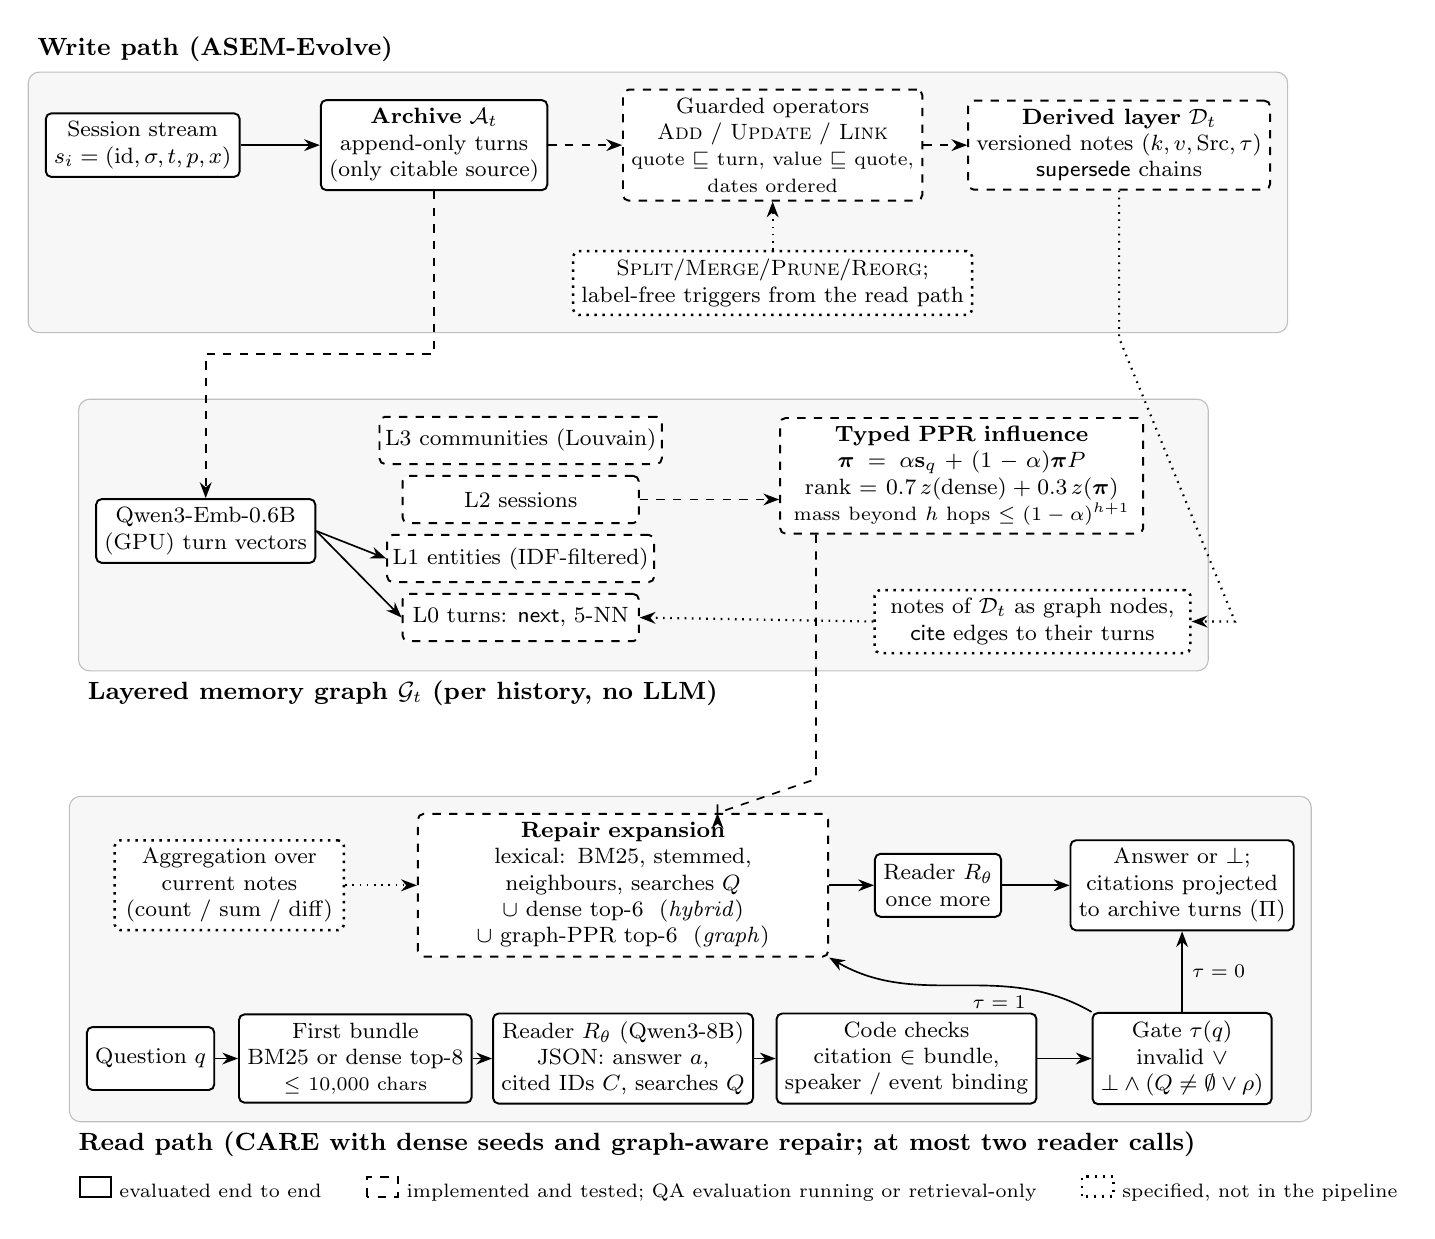
\begin{tikzpicture}

% ================= Write path (top) =================
\node[ok]  (stream)  at (0.2, 0)   {Session stream\\$s_i=(\mathrm{id},\sigma,t,p,x)$};
\node[ok]  (archive) at (3.9, 0)   {\textbf{Archive} $\mathcal{A}_t$\\append-only turns\\(only citable source)};
\node[run] (ops)     at (8.2, 0)   {Guarded operators\\\textsc{Add} / \textsc{Update} / \textsc{Link}\\{\scriptsize quote $\sqsubseteq$ turn, value $\sqsubseteq$ quote,}\\{\scriptsize dates ordered}};
\node[run] (derived) at (12.6, 0)  {\textbf{Derived layer} $\mathcal{D}_t$\\versioned notes $(k,v,\mathrm{Src},\tau)$\\\textsf{supersede} chains};
\node[spec] (more)   at (8.2, -1.75) {\textsc{Split}/\textsc{Merge}/\textsc{Prune}/\textsc{Reorg};\\label-free triggers from the read path};
\draw[arr]  (stream) -- (archive);
\draw[darr] (archive) -- (ops);
\draw[darr] (ops) -- (derived);
\draw[sarr] (more) -- (ops);
\begin{scope}[on background layer]
  \node[band, fit=(stream)(archive)(ops)(derived)(more)] (wband) {};
\end{scope}
\node[title, anchor=south west] at (wband.north west) {Write path (\textsc{ASEM-Evolve})};

% ================= Layered memory graph (middle) =================
\node[run, layer] (l3) at (5.0, -3.75) {L3 communities (Louvain)};
\node[run, layer] (l2) at (5.0, -4.50) {L2 sessions};
\node[run, layer] (l1) at (5.0, -5.25) {L1 entities (IDF-filtered)};
\node[run, layer] (l0) at (5.0, -6.00) {L0 turns: \textsf{next}, 5-NN};
\node[ok] (enc) at (1.0, -4.9) {Qwen3-Emb-0.6B\\(GPU) turn vectors};
\node[run, text width=44mm] (ppr) at (10.6, -4.20) {\textbf{Typed PPR influence}\\$\boldsymbol\pi=\alpha\mathbf{s}_q+(1-\alpha)\boldsymbol\pi P$\\rank $=0.7\,z(\text{dense})+0.3\,z(\boldsymbol\pi)$\\{\scriptsize mass beyond $h$ hops $\le(1-\alpha)^{h+1}$}};
\node[spec, text width=38mm] (notesL) at (11.5, -6.05) {notes of $\mathcal{D}_t$ as graph nodes,\\\textsf{cite} edges to their turns};
\draw[arr]  (enc.east) -- (l1.west);
\draw[arr]  (enc.east) -- (l0.west);
\draw[darr] (l2.east) -- (ppr.west |- l2.east);
\draw[sarr] (notesL.west) -- (l0.east);
\draw[darr] (archive.south) -- (archive.south |- 0,-2.65) -- (enc.north |- 0,-2.65) -- (enc.north);
\draw[sarr] (derived.south) -- (derived.south |- 0,-2.45) -- ($(notesL.east)+(0.55,0)$ |- 0,-2.45)
            -- ($(notesL.east)+(0.55,0)$) -- (notesL.east);
\begin{scope}[on background layer]
  \node[band, fit=(l3)(l0)(enc)(ppr)(notesL)] (gband) {};
\end{scope}
\node[title, anchor=north west] at (gband.south west) {Layered memory graph $\mathcal{G}_t$ (per history, no LLM)};

% ================= Read path (bottom) =================
% repair row
\node[spec, text width=27mm] (agg)  at (1.3, -9.4) {Aggregation over\\current notes\\(count / sum / diff)};
\node[run, text width=50mm] (expand) at (6.3, -9.4) {\textbf{Repair expansion}\\lexical: BM25, stemmed, neighbours, searches $Q$\\$\cup$ dense top-6 \ (\emph{hybrid})\\$\cup$ graph-PPR top-6 \ (\emph{graph})};
\node[ok] (reader2) at (10.3, -9.4) {Reader $R_\theta$\\once more};
\node[ok] (out) at (13.4, -9.4) {Answer or $\bot$;\\citations projected\\to archive turns ($\Pi$)};
% main row
\node[ok] (q)      at (0.3, -11.6) {Question $q$};
\node[ok] (seed)   at (2.9, -11.6) {First bundle\\BM25 or dense top-8\\{\scriptsize $\le$ 10{,}000 chars}};
\node[ok] (reader) at (6.3, -11.6) {Reader $R_\theta$ (Qwen3-8B)\\JSON: answer $a$,\\cited IDs $C$, searches $Q$};
\node[ok] (check)  at (9.9, -11.6) {Code checks\\citation $\in$ bundle,\\speaker / event binding};
\node[ok] (gate)   at (13.4, -11.6) {Gate $\tau(q)$\\invalid $\lor$\\$\bot\land(Q\neq\emptyset\lor\rho)$};
\draw[arr] (q) -- (seed);
\draw[arr] (seed) -- (reader);
\draw[arr] (reader) -- (check);
\draw[arr] (check) -- (gate);
\draw[arr] (gate) -- node[right, font=\scriptsize]{$\tau=0$} (out);
\draw[arr] (gate.north west) to[out=150, in=-30] node[below, font=\scriptsize, pos=0.35]{$\tau=1$} (expand.south east);
\draw[arr] (expand) -- (reader2);
\draw[arr] (reader2) -- (out);
\draw[sarr] (agg) -- (expand);
\draw[darr] (8.75,0 |- ppr.south) -- (8.75,-8.05) -- ($(expand.north)+(1.2,0)$ |- 0,-8.05) -- ($(expand.north)+(1.2,0)$);
\begin{scope}[on background layer]
  \node[band, fit=(agg)(expand)(reader2)(out)(q)(seed)(reader)(check)(gate)] (rband) {};
\end{scope}
\node[title, anchor=north west] at (rband.south west) {Read path (\textsc{CARE} with dense seeds and graph-aware repair; at most two reader calls)};

% ================= Legend =================
\node[anchor=north west, font=\scriptsize, align=left] at ($(rband.south west)+(0,-0.55)$) {%
\tikz{\draw[line width=0.7pt] (0,0) rectangle (4mm,2.5mm);}\ evaluated end to end\qquad
\tikz{\draw[dashed, line width=0.7pt] (0,0) rectangle (4mm,2.5mm);}\ implemented and tested; QA evaluation running or retrieval-only\qquad
\tikz{\draw[dotted, line width=0.9pt] (0,0) rectangle (4mm,2.5mm);}\ specified, not in the pipeline};

\end{tikzpicture}
\end{document}
